\documentclass[11pt]{article}

\usepackage{hyperref,amsmath,amssymb,amsthm,bm,graphicx}
\usepackage[parfill]{parskip}
\usepackage[margin=1in]{geometry}
\graphicspath{ {images/} }


\newtheoremstyle{quest}{\topsep}{\topsep}{}{}{\bfseries}{}{ }{\thmname{#1}\thmnote{ #3}.}
\theoremstyle{quest}
\newtheorem*{definition}{Definition}
\newtheorem*{theorem}{Theorem}
\newtheorem*{question}{Problem}
\newtheorem*{exercise}{Exercise}
\newtheorem*{challengeproblem}{Challenge Problem}

\newcommand{\name}{CS 189: Introduction to Machine Learning}
\newcommand{\hw}{4}
\newcommand{\duedate}{March 31, 2016 at 11:59pm}

\title{
\Large \name
\\\vspace{10pt}
\Large Homework \hw
\\\vspace{10pt}
\large Due: \duedate}
\date{}
\author{}

\markright{\name\hfill Homework \hw\hfill}

%% If you want to define a new command, you can do it like this:
\newcommand{\Q}{\mathbb{Q}}
\newcommand{\R}{\mathbb{R}}
\newcommand{\Z}{\mathbb{Z}}
\newcommand{\C}{\mathbb{C}}

%% If you want to use a function like ''sin'' or ''cos'', you can do it like this
%% (we probably won't have much use for this)
% \DeclareMathOperator{\sin}{sin}   %% just an example (it's already defined)
\renewcommand\qedsymbol{$\blacksquare$}

\newcommand{\mysection}[2]{
    \setcounter{section}{#1}
    \section*{#2}
    \addcontentsline{toc}{section}{#2}
}
\renewcommand{\subsection}[2]{
    \setcounter{subsection}{#1}
    \section*{#2}
    \addcontentsline{toc}{subsection}{#2}
}

\begin{document}
\maketitle
\vspace{2ex}
\begin{picture}(0,0)
\put(0,180){\textbf{Name: UTSAV BARAL} \hspace{6cm} \textbf{Student ID: 25694452}}
\end{picture}
\vspace{-1.25in}\\[5ex]

% =============================================================
\mysection{1}{Problem 1: Ridge Regression}
  \subitem(a) We will first expand the matrix equation given to us, and see how it simplifies. And we will set the gradient, $\nabla J = 0$ and solve for values of $w $ and $ \alpha$ which minimize this modified squared loss function. Starting with the cost function: $J(\mathbf{w},\alpha) = (\mathit{X}\mathbf{w} + \alpha \mathbf{1} - \mathbf{y})^t (\mathit{X}\mathbf{w} + \alpha \mathbf{1} - \mathbf{y}) + \lambda\mathbf{w}^t\mathbf{w}$ We can see right off the bat that the complicated looking part with the transpose of the expression multiplied with itself is the expression describing the squared loss, and the added expression, is how ridge regression attempts to keep variance low by punishing very large weight values, and thus helping with potential overfitting problems. Specifically, we have that:
\begin{equation}
  \begin{split}
    \nonumber
    J(\mathbf{w}, \alpha) &= (\mathit{X}\mathbf{w} + \alpha \mathbf{1} - \mathbf{y})^t (\mathit{X}\mathbf{w} + \alpha \mathbf{1} - \mathbf{y})+ \lambda\mathbf{w}^t\mathbf{w}\\
    &= \left[\begin{matrix}
          X_{11}w_1 + \hdots + X_{1d}w_d + \alpha - y_1\\
          X_{21}w_1 + \hdots + X_{2d}w_d + \alpha - y_2\\
          \vdots\\
          X_{n1}w_1 + \hdots + X_{nd}w_d + \alpha - y_n\\   
        \end{matrix}\right]^t
        \left[\begin{matrix}
                  X_{11}w_1 + \hdots + X_{1d}w_d + \alpha - y_1\\
                  X_{21}w_1 + \hdots + X_{2d}w_d + \alpha - y_2\\
                  \vdots\\
                  X_{n1}w_1 + \hdots + X_{nd}w_d + \alpha - y_n\\   
        \end{matrix}\right] + (\lambda w_1^2 + \hdots + \lambda w_d)\\
        &= \sum_{i=1}^{n} (X_{i1}w_1 + \hdots + X_{id}w_d + \alpha - y_i)^2 \; + (\lambda w_1^2 + \hdots + \lambda w_d)
  \end{split}
\end{equation}
Now that its actually readable, we can take the partials with respect to $\mathbf{w}$ and $\alpha$ and set equal to zero to find where the grad is 0 and where we have a critical minimum point. 
We can write the equation again, in terms of a sum of all the row vectors:
\begin{equation}
  \begin{split}
    \nonumber
    J &= \sum_{i=1}^{n} (X_{i}\mathbf{w} + \alpha - y_i)^2 \;+\; (\lambda w_1^2 + \hdots + \lambda w_d)\\
    \frac{\partial J}{\partial \mathbf{w}} &= \sum_{i=1}^{n} 2 \left[\begin{matrix}X_{i1}\\\vdots\\X_{id}\end{matrix}\right](X_{i}\mathbf{w} + \alpha - y_i) \;+\; 2\lambda\left[\begin{matrix}w_1\\\vdots\\w_d\end{matrix}\right]
  \end{split}
\end{equation}
Since each $X_i$ row ends up geting transposed, the whole sum can just be written as a big matrix with where the design matrix gets transposed and left multiplied to acheive the sum. We then expand the resulting expression out:
\begin{equation}
  \begin{split}
    \nonumber
    \frac{\partial J}{\partial \mathbf{w}} &= 2\mathit{X}^t\mathit{X}\mathbf{w} + 2\mathit{X}^t\alpha - 2\mathit{X}^ty \;+\; 2\lambda \mathbf{w}
  \end{split}
\end{equation}
Setting this simplified expression to 0, we then get that:
\begin{equation}
  \begin{split}
    \nonumber
    \mathit{X}^ty &= \mathit{X}^t\mathit{X}\mathbf{w} + \mathit{X}^t\alpha + \lambda \mathbf{w}
  \end{split}
\end{equation}
Another simplification can be made, since $X^t\alpha$ contains elements that are the column sums of the design matrix times some constant, this must be zero! Since we are given that the mean of $x$ is 0. Thus we can rewrite again, factor the \textbf{w} vector and get our answer for \textbf{w}:
\begin{equation}
  \begin{split}
    \nonumber
    \mathit{X}^ty &= \mathit{X}^t\mathit{X}\mathbf{w} + \lambda \mathbf{w}\\
    \mathit{X}^ty &= \mathit{X}^t\mathit{X}\mathbf{w} + (\lambda \mathbf{I})\mathbf{w}\\
    \mathit{X}^ty &= (\mathit{X}^t\mathit{X} + \lambda \mathbf{I})\mathbf{w}\\
    \therefore \mathbf{w} &= (\mathit{X}^t\mathit{X} + \lambda \mathbf{I})^{-1}\mathit{X}^ty \qed
  \end{split}
\end{equation}
Finding the value for $\alpha$ is pretty easy since we have a just a normal partial derivative without complicated vectors, we set the partial $= 0$ and simplify:
\begin{equation}
  \begin{split}
    \nonumber
    \frac{\partial J}{\partial \alpha} &= 2\sum_{i=1}^{n} X_i \mathbf{w} \;+\; 2(n\cdot\alpha) + 2\sum_{i=1}^{n} -y_i = 0\\
    \sum_{i=1}^{n} y_i  &= \sum_{i=1}^{n} X_i \mathbf{w} \;+\; (n\cdot\alpha)
  \end{split}
\end{equation}
We are treating w as a constant, since this is a partial derivative, and again, since we know that the mean of x is 0, that whole sum just drops out, and we are left with:
\begin{equation}
  \begin{split}
    \nonumber
    \sum_{i=1}^{n} y_i  &= n\cdot\alpha\\
    \therefore \alpha &= \frac{1}{n}\sum_{i=1}^{n} y_i = \bar{y} \qed
  \end{split}
\end{equation}
\subitem(b)
  \subsubitem i. See APPENDIX A.
  \subsubitem ii. [$\lambda=106$ to $\lambda=136$] were where good ranges of hyperparamaters occured. The residual sum os squared on this malication set was...
  \subsubitem iii. Here is a plot generated using python (see APPENDIX B for code):

\newpage
\begin{question}[2: Logistic Regression] \end{question}
\textit{***See APPENDIX C for Code***}\\[5ex]
Design Matrix (\textbf{X}) = $\left[\begin{matrix}0&3&1\\ 1&3&1\\ 0&1&1\\1&1&1\end{matrix}\right]$;\;\;Labels(\textbf{y}) = $\left[\begin{matrix}1\\1\\0\\0\end{matrix}\right]$;\;\;$\mathbf{w}^{(0)} = \left[\begin{matrix}-2\\1\\0\end{matrix}\right]$
\subitem(a.) $R(\mathbf{w}^{(0)}) = 1.9883724141284105$
\subitem(b.) $\mu^{(0)} = \left[ \begin{matrix} 0.95257413\\0.73105858\\0.73105858\\0.26894142 \end{matrix}\right]$
\subitem(c.) $\mathbf{w}^{(1)} = \left[\begin{matrix} -2\\0.94910188\\-0.68363271 \end{matrix}\right]$
\subitem(d.) $R(\mathbf{w}^{(1)}) = 1.720617095621304$
\subitem(e.) $\mu^{(1)} = \left[ \begin{matrix} 0.89693957 \\ 0.54082713\\0.56598026\\0.15000896 \end{matrix}\right]$
\subitem(f.) $\mathbf{w}^{(2)} = \left[\begin{matrix} -1.69083609\\1.91981257\\-0.83738862 \end{matrix}\right]$
\subitem(g.) $R(\mathbf{w}^{(2)}) = 1.8546997847922464$
\subitem(h.) $\mu^{(2)} = \left[ \begin{matrix} 0.99276849\\0.96199213\\0.74695242\\0.35242149 \end{matrix}\right]$

\newpage
\begin{question}[3: Spam classification using Logistic Regression] \end{question}

\subitem(1.) Batch Gradient Descent, 60 iterations until it started converging:\\
	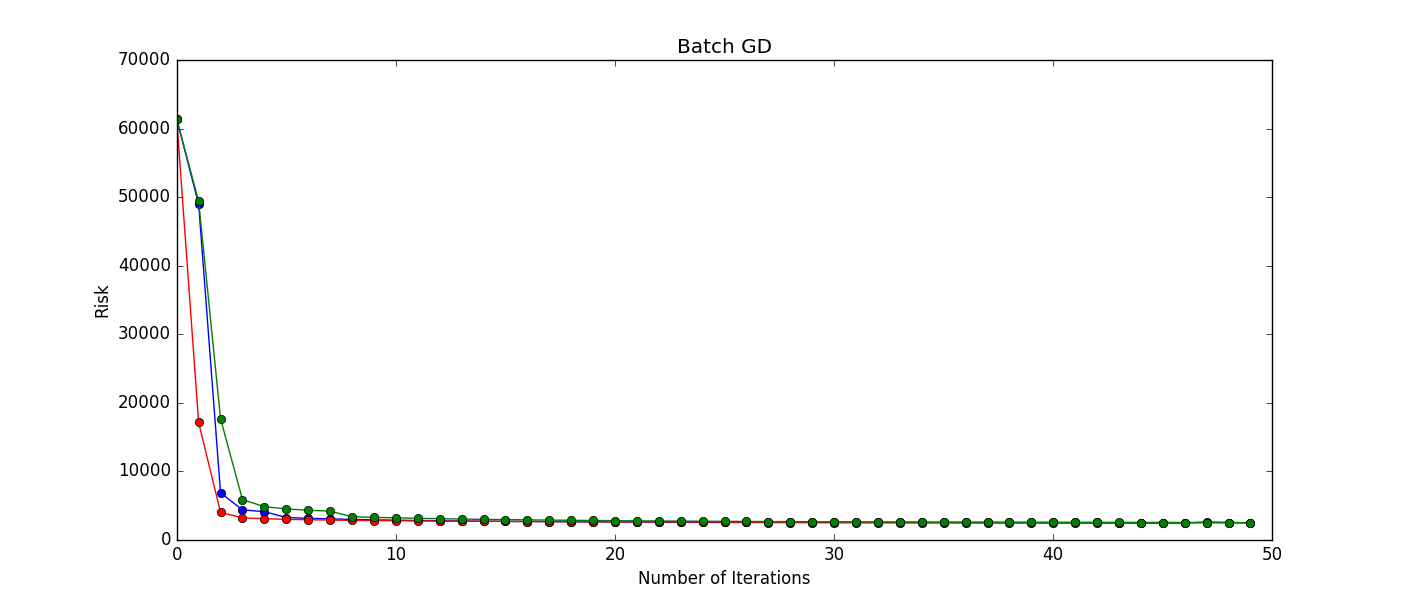
\includegraphics[scale=.5]{batch_gd}
\subitem(2.) Stochastic Gradient Descent,(Title Says Batch on Accident):\\
	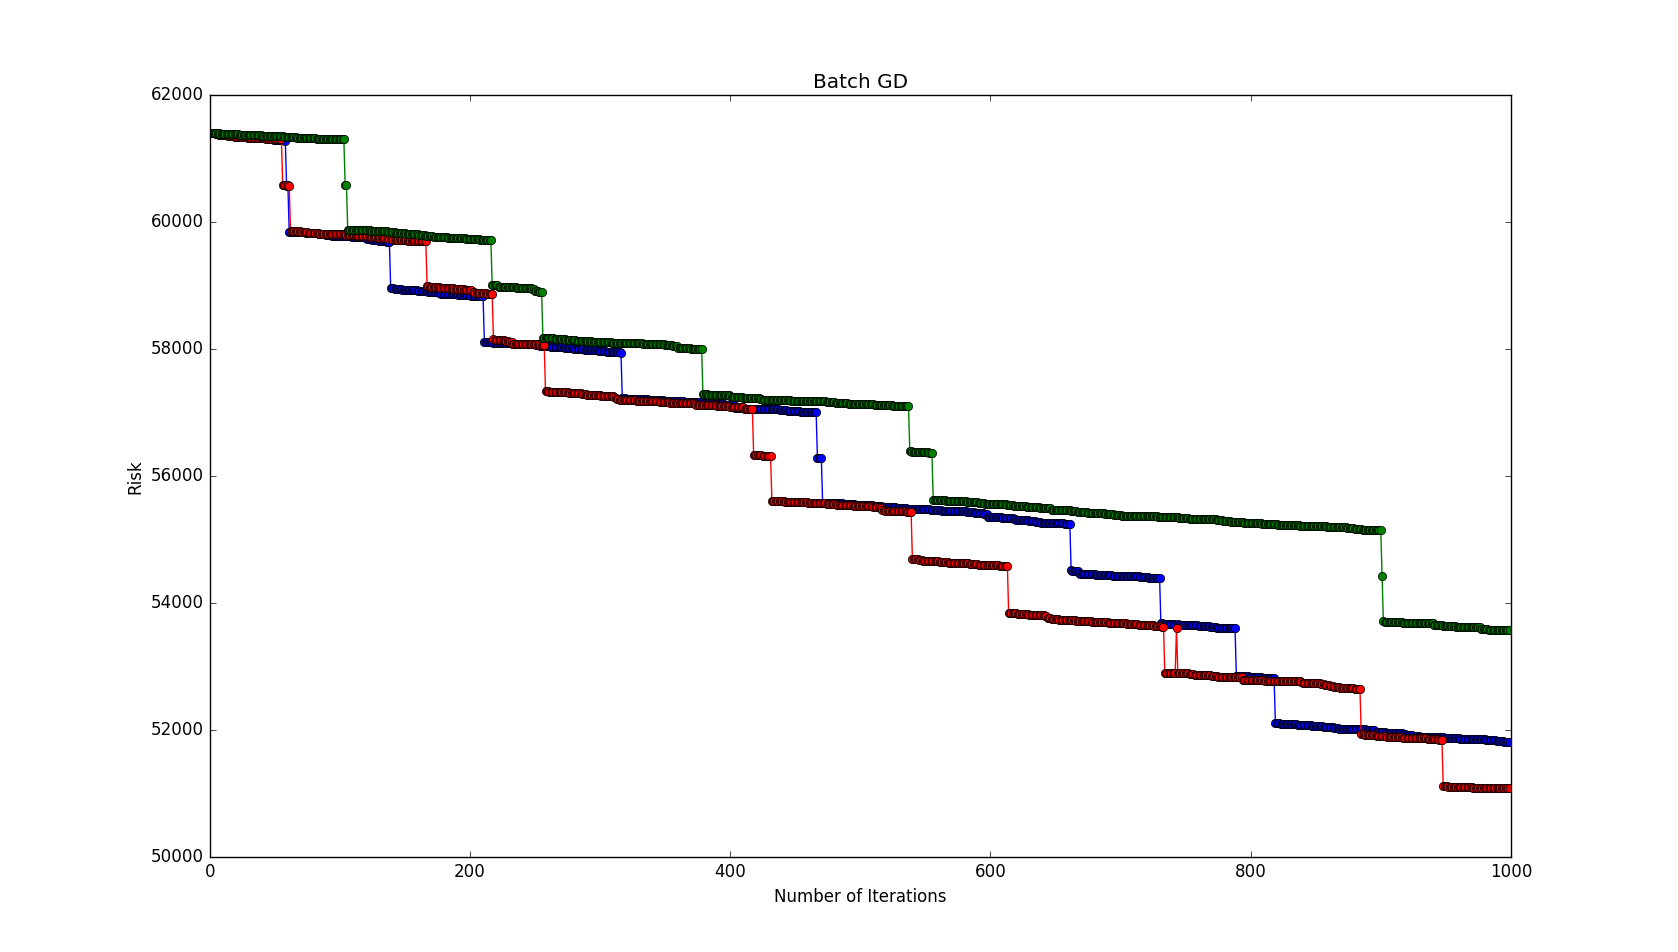
\includegraphics[scale=.43]{stochastic}\\[10ex]
\subitem(3.) Stochastic Gradient Descent, with Decaying Learning Rate:\\
	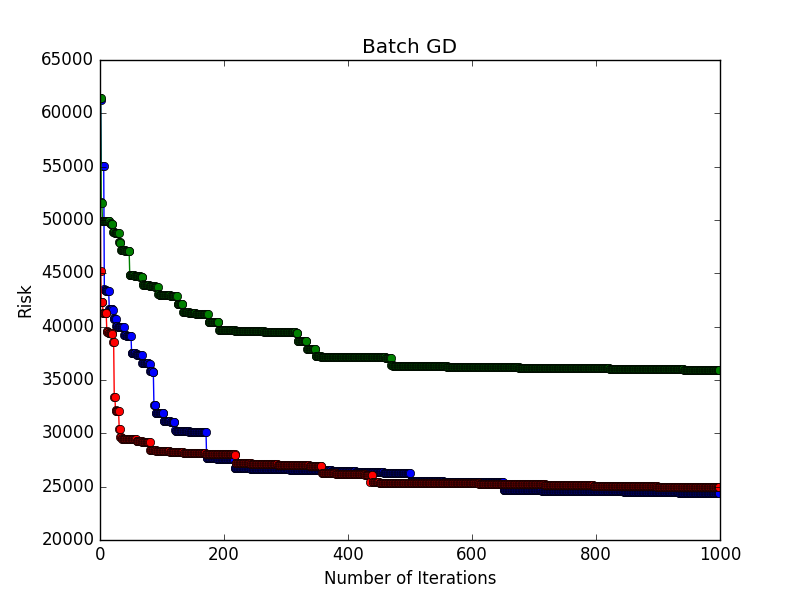
\includegraphics[scale=.6]{stochastic_decay}\\[3ex]
\subitem(4.)\\[3ex]
\subitem(5.) Clearly, batch gradient descent worked the best, maybe due to better hyperparameter maniupulation, or possible/probably error in code of the other methods. I will use batch gradient descent with log preprocessing for kaggle. SCORE=0.76422

\newpage
\begin{question}[4: Revisiting Logistic Regression] \end{question}
\subitem(a) Replacing $\tanh (z)$ with the corresponding function we have that $g(z) = \frac{(2s(2z) + 1) - 1}{2} = s(2z)$ So we can just simplify this expression:
\begin{equation}
	\begin{split}
		\nonumber
		s(2z) &= \frac{1}{1 + e^{-2z}} = \frac{1}{1 + e^{-2z}} \cdot \frac{e^z}{e^z}\\[3ex]
		&= \frac{e^z}{e^z + e^{-z}} = \frac{2e^z}{2(e^z + e^{-z})} = \frac{e^z - e^{-z} + e^z + e^{-z}}{2(e^z + e^{-z})}\\[3ex]
		&= \frac{e^z - e^{-z}}{2(e^z + e^{-z})} + \frac{e^z + e^{-z}}{2(e^z + e^{-z})}\\[4ex]
		&= \frac{e^z - e^{-z}}{2(e^z + e^{-z})} + \frac{1}{2} \qed
	\end{split}
\end{equation}
\subitem(b)
With simple application of the chain rule, we see that $\frac{dg}{dz} = \frac{1}{2}\frac{dh}{dz} = 2 \frac{ds}{dz}$ We can expand this expression to see that:
\begin{equation}
	\begin{split}
		\nonumber
		2 \frac{ds}{dz} = \frac{e^{-z}}{(1+e^{-z})^2} = 
	\end{split}
\end{equation}
\subitem(c)
\newpage
\begin{question}[5: Real World Spam Classification] \end{question}

\end{document}
